% This example An LaTeX document showing how to use the l3proj class to
% write your report. Use pdflatex and bibtex to process the file, creating 
% a PDF file as output (there is no need to use dvips when using pdflatex).

% Modified 

\documentclass{l3proj}
\begin{document}
\title{Team V - How Not To Kill Your Dog}
\author{Ross Adam \\
        Andrew Gardner \\
        Nicole Kearns \\
        Mamas Nicolaou \\
        Asset Sarsengaliyev}
\date{18 March 2013}
\maketitle

\tableofcontents

\chapter{Background}
\label{background}

This section discusses several different existing artifacts, both medical applications and other revision tools. These applications were selected to provide inspiration for our own application design, specifically assessing the current tools within the market and how each displays their content to the user.

\section{Investigation of Existing Artifacts}


There are a few similar tools and learning resources available for vetinary students. This section discusses some of the current tools and a few tools which our client, Dr Fiona Dowell, has shown us in order to give us an idea of what she wanted for the application.

\subsection{Medical Helper Applications}


\subsubsection{NHS Adult Drug Calculations}

\begin{figure}[!htb]
\minipage{0.32\textwidth}
  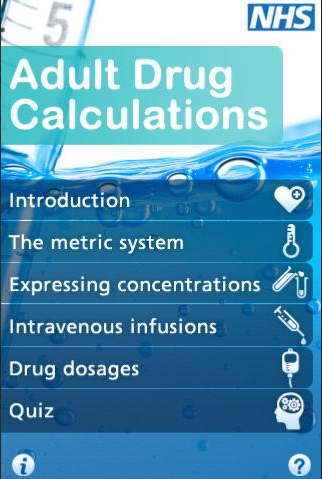
\includegraphics[width=\linewidth]{/users/level3/0902059k/Level3/TP3/team-project/Dissertation/images/NHSDrugApp/NHSDrugApp2.png}
\endminipage\hfill
\minipage{0.32\textwidth}
  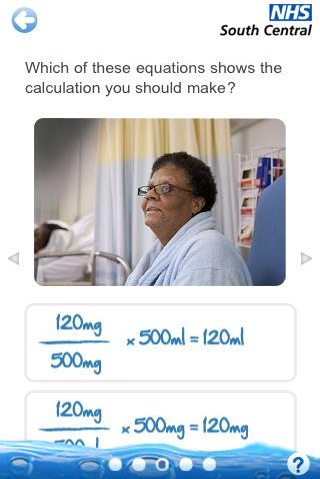
\includegraphics[width=\linewidth]{/users/level3/0902059k/Level3/TP3/team-project/Dissertation/images/NHSDrugApp/NHSDrugApp4.png}
\endminipage
\end{figure}


The NHS Adult Drug Calculations is a smartphone based learning tool aimed at nurses and midwives who are newly qualified or returning to practice. The tool allows the user to browse through different topics. Within each topic, there are a number of slides providing the user with the information and theory behind the calculations, and then has a few "Check your knowledge" slides containing multiple choice questions to test the user on what they have read. The interface is very simple and easy to use. The main menu allows the user to simply select which topic they qish to go over. Within each topic, there are arrows on each page which will allow the user to navigate back and forward between the pages and there are breadcrumbs at the bottom of each page indicating how far through the topic they are.  There is also an arrow at the top left-hand corner which will allow the user to return to the main menu at any point. One feature which is particularly useful to new users is the help button, which informs the user how to use the application. This application is very similar to the application which our client would like for the vetinary students.

\subsubsection{Vet Calculator}

\begin{figure}[!htb]
\minipage{0.32\textwidth}
  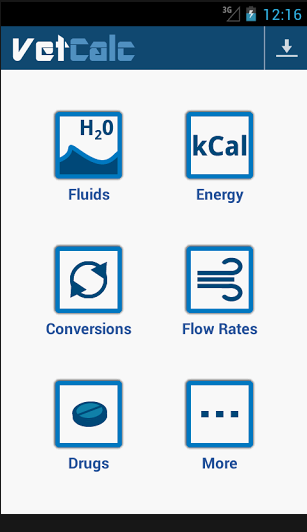
\includegraphics[width=\linewidth]{/users/level3/0902059k/Level3/TP3/team-project/Dissertation/images/VetCalcApp/VetCalcApp1.png}
\endminipage\hfill
\minipage{0.32\textwidth}
  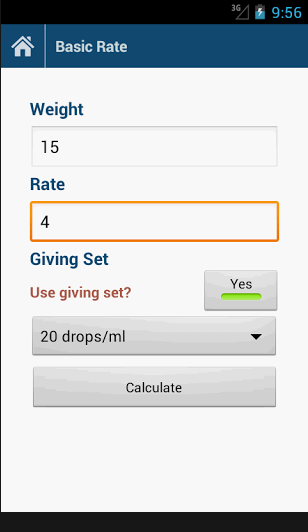
\includegraphics[width=\linewidth]{/users/level3/0902059k/Level3/TP3/team-project/Dissertation/images/VetCalcApp/VetCalcApp3.png}
\endminipage\hfill
\minipage{0.32\textwidth}%
  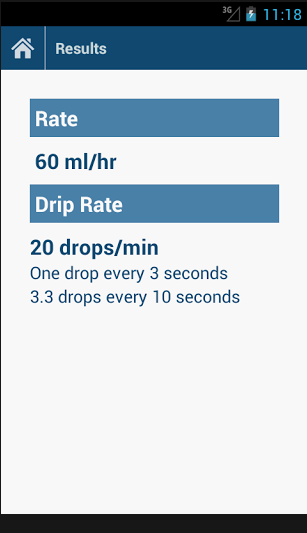
\includegraphics[width=\linewidth]{/users/level3/0902059k/Level3/TP3/team-project/Dissertation/images/VetCalcApp/VetCalcApp4.png}
\endminipage
\end{figure}

VetCalc is an android based tool aimed at verterinarians, students, nurses and technicians, which allows the user to enter the necessary details, such as weight; dose; formulation; volume of fluid; etc. and will produce the result for the user. The interface for the vet calculator is very simple and easy to use. The menu is a simple grid-layout of different topics and sections for drug calculations. Within each topic, the user has to simply enter the necessary details into the clearly labelled text boxes and click 'Calculate' in order to get the result of the calcuation. On each page, there is a home button which will easily allow the user to return to the main menu at any point. This application is useful for users who simply need to get the results of a calculation. However, out client wants an application that will teach the students how to carry out the calculations and not simply produce the result for them as they will need to know how to carry out these calculations throughout their career.

\subsection{Revision Tools}

Before desgining our own application the team agreed that we should
research existing tools for revision. The following were suggested as
members had had some experience using them. 

\subsubsection{Bitesize}
The Bitesize revision tool is a service provided by the BBC which
operates in the user's web browser. It is a simple implementation of
linked webpages that cover a variety of subjects from across the UK
national curriculum. The team chose to research the Bitesize system
because several of the Scottish Students had used it before and found
it helpful for their studies at high school. First we decided to analyse how the
content is displayed within the tool.\\

\begin{figure}[!htb]
\caption{Bitesize Layout}
 \centering
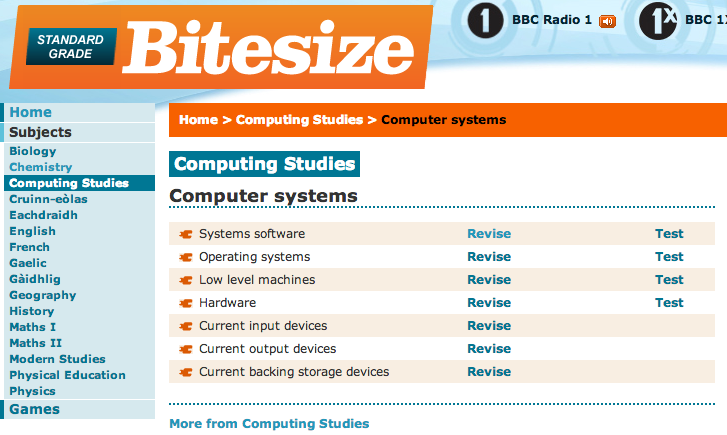
\includegraphics[width=0.9\textwidth]{/users/level3/0902059k/Level3/TP3/team-project/Dissertation/images/Bitesize/BitesizeLayout.png}
\end{figure}

Figure 1.1 shows the typical layout of a Bitesize page: each page of
content is framed by the Bitesize logo (implemented as a clickable image that
returns the user to the main page) and on the right of the screen is
the index for various subjects allowing for quick navigation.\\

\begin{figure}[!ht]
\caption{Bitesize Content}
 \centering
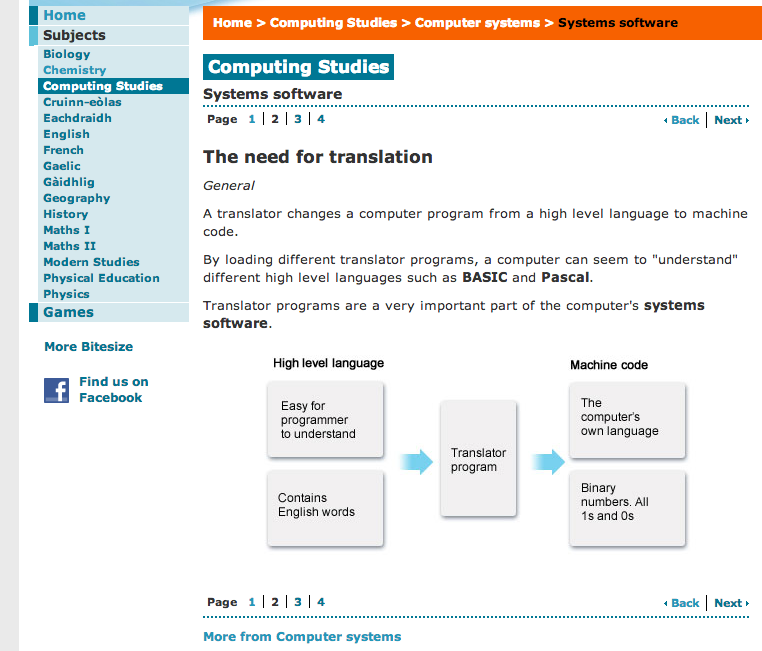
\includegraphics[width=0.9\textwidth]{/users/level3/0902059k/Level3/TP3/team-project/Dissertation/images/Bitesize/BitesizeContent.png}
\end{figure}

A consistent frame is a concept that Team V also wanted to achieve
within our own design. Instead of a bitesize logo we would use the
Veterinary School logo which would make our application appear more
professional. Our index page will feature links to different topics
for fast navigation for experienced users.\\


Figure 1.2 illustrates how each page is displayed in the tool. Content
is simply loaded into the page in the center and navigation is
achieved by clicking specific buttons. Our goal is to have a simple
slider to sequentially navigate pages.\\
\newpage
\subsubsection{Hot Potatoes}

The second system Team V assessed was Hot Potatoes, a simple quiz
creation system that allows users to create online quizzes which they
can then publish for other users to interact with.\\ 

\begin{figure}[!htb]
\caption{Hot Potatoes Program}
 \centering
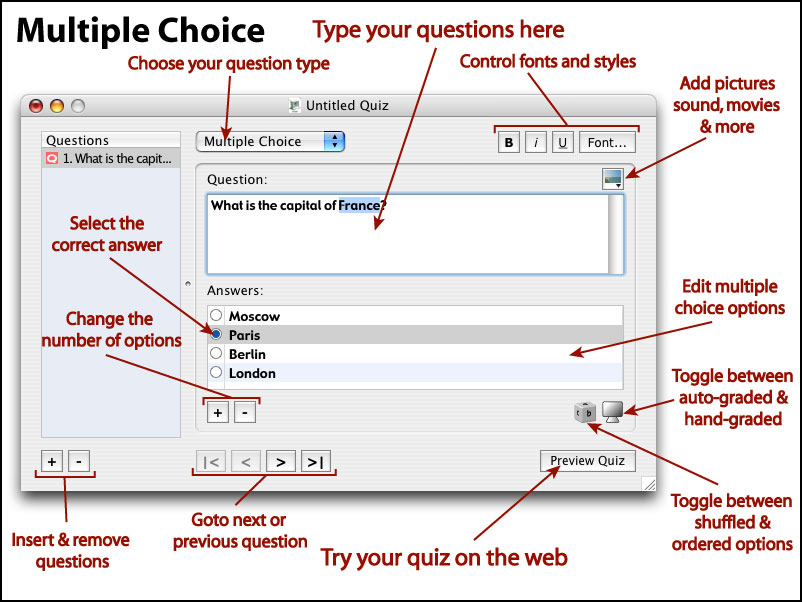
\includegraphics[width=0.9\textwidth]{/users/level3/0902059k/Level3/TP3/team-project/Dissertation/images/HotPotatoes/HotPotatoesQuestion.jpg}
\end{figure}

The system itself is a comprehensive suite of features and programs
that can produce different types of quizzes: multiple choice; image
matching and several more.\\

The included figure shows how a user can create a multiple choice question. This is much more complex than our implementation will be but it gave us an idea of how to make the process streamlined and easier for the user to work with.\\ 

The client has requested a system that includes questions which can be
answered at the same time as the course content is being
displayed. This would hopefully ensure the student retained the
information better than simply reading the slides. Our system will
only allow multiple choice questions to be created.

\end{document}
